% elemCell.tex      pdflatex ZhCvGo15
% Diffuse globally, compute locally: a cyclist tale
% Tingnan Zhang, Daniel I. Goldman and Predrag Cvitanovi\'c

%\section{Cycles in the elementary cell}
%\label{s-elemCell}


The computation of diffusion coefficient \refeq{eq-diff-ec} requires
the knowledge of periodic orbits. In the Lorentz gas system, some
simple orbits may be obtained by direct observation. For example, the
shortest periodic orbit involves the particle reflecting between a disk
and one of its nearest neighbors; The motion that travels to and
bounces back from the second nearest disk is also trivial. On the
other hand, longer orbits (measured by $n_p$, which we refer to as the
topological length) are generally complicated structures in space, and
the number of orbits increase exponentially with length.  While
numerical techniques that involves root finding, e.g., Newton's method,
may find a few long periodic orbits, it is impossible to generate
all orbits, because the convergence depends sensitively on the initial
conditions and step lengths.

Instead, we explore the \emph{symbolic dynamics} associated with the
hyperbolic system. The idea is to identify each periodic orbit with a
unique sequence of symbols, drawn from a finite alphabet set.
Intuitively speaking, a symbol may characterize a certain pattern of
the dynamics. Once the symbol set is determined, we may enumerate all
possible periodi orbits and eventually pin them down.

We use the symbolic dynamics developed in \refref{CGS92} and briefly
review the concepts here. With imposed finite horizon there are 12
possible ways of jump from a disk
(\reffig{fig-diskDirectionsElCell}\,(a)). Any trajectory in the full
space can always be constructed from a series of flights, each belongs
to the 12 ``signature jumps''. In particular, a periodic orbit in the
elementary cell is represented as a repeatable string of such symbols.
For example, the bouncing mode between nearest disks is written as
\cycle{06}, meaning that the periodic orbit is consisted of two
successive flights, one traveling towards right (symbol $0$) and the
next reflecting backwards (symbol $6$).

Periodic orbits in the elementary cell can either be stationary in the
full space that goes back to its original place after completing a
full cycle (e.g., \cycle{06} that represents the bouncing of the
particle between two nearest disk); or can be in a running mode that
generates a net displacement along the trajectory (e.g., \cycle{05},
\reffig{fig-diskDirectionsElCell}\,(a) and (c). The stationary cycles
``trap'' the  particle locally for a finite amount of time while the
running cycles advance it. The final diffusion \refeq{eq-diff-ec}
can be conceptually understood as the result of competition between
the two type of cycles.

With the symbolic dynamics, we then use the least action principle to
compute the periodic orbits\rf{DasBuch}. In a planetary Hamiltonian
billiard system, the Maupertuis' principle indicates that the
traveling length along a cycle is minimized. We can solve the problem
by optimizing the total free flight distance with the constraint that
links have to connect the specific disks visited along the orbit.

\begin{figure}
  \begin{center}
    (a)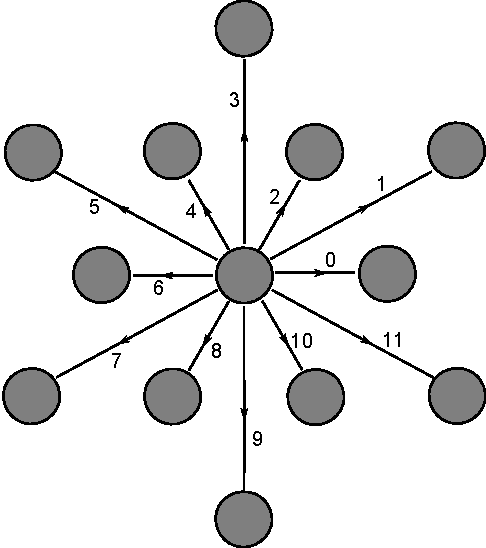
\includegraphics[width=0.27\textwidth]{diffuseDiskDirectionsElCell}
    (b)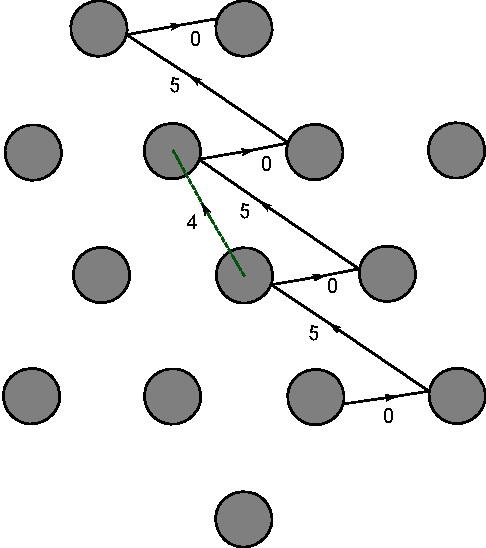
\includegraphics[width=0.27\textwidth]{diffuseDiskDirecsElCell05}
    (c)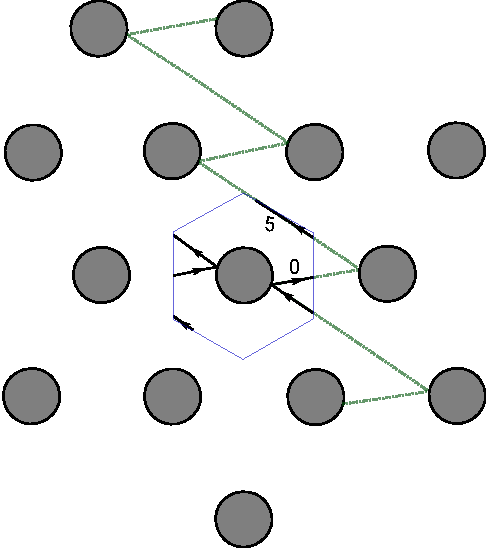
\includegraphics[width=0.27\textwidth]{diffuseDiskDirecsElCell05red}
  \end{center}
  \caption{\label{fig-diskDirectionsElCell}
  Elementary cell symbolic dynamics is obtained by counterclockwise
  labeling the translation vectors connecting the center of the current
  disk to the center of  the next disk. (a) The finite horizon is here
  imposed by limiting jumps from  the center cell to six short jumps
  (even labels $0, 2,\cdots,10$) and six `long' jumps (odd labels $1,
  3,\cdots,11$). (b) Running mode  \cycle{05} advances by $\hn_4$ per
  period. (c) In the elementary cell this is  a \po\ \cycle{05} of
  topological length 2.
  }
\end{figure}

Some confidence can be gained at this point by applying the above
formula~\refeq{eq-diff-ec} to a trivial system. For a simple example,
see the chain of baker's maps chain of coupled baker maps studied in
\refref{Gaspard92}.

In this case there are only four fixed points, all with stability
$\Lambda_p=1/2$, two of which give rise to the translations
$\hn_{p}=\pm 1$. As the system is uniformly hyperbolic, all curvature
terms are identically zero, and the fixed points substituted into
\refeq{eq-diff-ec} yield immediately the correct result $D=1/4$.
